%\documentclass{llncs}
\documentclass[spanish]{llncs}
%\usepackage{makeidx}
%\usepackage{amsfonts}
%\usepackage{amsmath}
%para incluir imagenes en png,jpg y pdf
\usepackage[pdftex]{graphicx}
%para usar texto coloreado
\usepackage{color}
%para tabla
\usepackage{multirow}
%\usepackage{setspace}
%\usepackage{verbatim}
%\usepackage{algorithm}
%\usepackage{algorithmic}

%\usepackage[T1]{fontenc}
\usepackage[utf8]{inputenc}
%\usepackage{babel}

   
\begin{document}\hyphenation{re-gis-tro de-sa-rro-llo va-rios e-va-lua-dor} 

\title{Un Framework Aspectual para la \colorbox{green}{Evaluación Automática} \\ de Usabilidad de Tareas
\thanks{Este trabajo fue apoyado por el proyecto PIA315/1 y parcialmente financiado por UNPA, Sta. Cruz, Arg.}}

\titlerunning{Un Framework Aspectual para la Evaluación Automática de Usabilidad de Tareas}
% abbreviated title (for running head) also used for the TOC unless
% \toctitle is used

\author{
Natalia Trejo , 
 Roberto Farias Y
 Sandra Casas    
}

\authorrunning{N. Trejo et al.}   % abbreviated author list (for running head)

% modified list of authors for the TOC (add the affiliations)

\tocauthor{
 Natalia Trejo (UARG - ITA),
 Roberto Farias  (UNPA - ITA),
 Sandra Casas (UARG - ITA)
}


\institute{
 Instituto de Tecnolog\'ia  Aplicada\\
 Universidad Nacional de la Patagonia Austral \\
 \email{ nbtrejo@gmail.com,fariasrobertoa@unpa.edu.ar, sicasas@yahoo.com} \\
} 


\maketitle

%-------------------------------------------------------------------------------

\begin{abstract}
La programación orientada a aspectos permite automatizar varias actividades de la evaluación de la usabilidad, en forma dinámica, transparente para el usuario y separada del código de las aplicaciones. A diferencia de otras propuestas, que se han centrado en pruebas que recolectan datos de bajo nivel de abstracción, este trabajo presenta un framework que permite realizar la evaluación de la usabilidad en aplicaciones de escritorio en el contexto de tareas de usuario. El framework consiste en un conjunto de módulos, aspectos y clases, que interactúan y se relacionan de manera tal de ser altamente reusable y sus requerimientos de especialización (configuración) son mínimos. 
\end{abstract}
{\em keywords:} usabilidad, framework, programación orientada a aspectos, AspectJ

\section{Introducción}
\label{sec:intro}

La evaluación de usabilidad [1] automática refiere a la posibilidad de disponer medios basados software para realizar alguna de las actividades en las que se descompone, captura de datos, análisis o crítica [2]. En lo que respecta a la captura de datos automatizada se ha caracterizado por usar archivos de logs. Sus ventajas son varias: soportan la ejecución de las pruebas en laboratorios de usabilidad o en el ambiente natural del usuario; son transparentes para los usuarios; permiten con facilidad obtener información de múltiples usuarios; permiten detectar errores comunes y actuales; etc. Los logs aportan gran cantidad de datos a los evaluadores de usabilidad, además de posibilitar la contrastación del comportamiento entre diferentes usuarios. Sin embargo, tienen desventajas, los logs generados por servidores webs o sistemas operativos, generan una gran cantidad de datos que resulta irrelevante para la evaluación de usabilidad, y son incapaces de registrar información específica. Por otro lado, añadir en las aplicaciones el código que realiza el logging de las actividades y  tareas de usuario que interesan al evaluador de usabilidad, implica invadir la estructura interna de las aplicaciones agregando cientos de líneas de código, cuya remoción posterior es muy compleja.

Las técnicas de separación de concerns [3], y en particular de la Programación Orientada a Aspectos (AOP) [4], proporcionan mecanismos para diseñar e implementar módulos de código que realicen la traza y el logging sin invadir y/o alterar la estructura interna de los sistemas. La posibilidad de realizar la recolección de los datos en forma dinámica, transparente para el usuario y separada del código de las aplicaciones a evaluar, ha provocado interés y varios enfoques se han presentado que aplican AOP a la evaluación de usabilidad. En particular aquellos propuestos para aplicaciones de escritos (WIMP) ofrecen esquemas para la evaluación a bajo nivel. Posibilitan la traza de los elementos o eventos de interfaces y/o errores pero sin un contexto de significado (tarea) para el evaluador. En consecuencia carecen de una relevancia real a la hora de interpretar los resultados y/o calcular métricas, y proporcionar información útil para emitir una opinión al evaluador de usabilidad. 

Luego de analizar los diseños presentados, se puede concluir que la razón radica en el hecho de que el concepto de “tarea” no es común en los vocabularios que participan de un escenario de evaluación de usabilidad y por ende no está presente en ambos contextos. En los sistemas software se representan los conceptos del dominio y lógica de negocios tales como: Cuenta, Cliente, Factura, Impuesto, Stock, etc., mientras que los evaluadores de usabilidad buscan identificar, analizar e interpretar  tareas de usuario. En los sistemas software  las “tareas de usuario” resultan ser entidades intangibles e inexistentes. Es por ello que los módulos (aspectos) que se diseñan e implementan para llevar adelante en forma automática las pruebas de la usabilidad, se restringen a los conceptos (entidades) existentes (métodos / atributos y clases del dominio), perdiéndose la concepción de la tarea. Planteamos como hipótesis, que sí es posible colocar en el centro la tarea, como concepto y como entidad, y por medio de aspectos conectarla al dominio y a los servicios que se requieran para la evaluación, entonces podrá ser identificada y analizada. En consecuencia se obtendrán datos que puedan ser interpretados a mayor nivel semántico y se lograrán resultados de mayor nivel de abstracción. 

En este trabajo presentamos un framework que permite realizar la evaluación de la usabilidad en aplicaciones de escritorio en el contexto de tareas de usuario. El framework consiste de un conjunto de módulos, aspectos y clases, que interactúan y se relación de manera tal de ser altamente reusable y sus requerimientos de especialización (configuración) son mínimos. 
Este trabajo se estructura de la siguiente manera, en la Sección 2 se describe brevemente el modelo de usabilidad soportado por el framework, en la Sección 3 se presenta el Framework, en la Sección 4 se exponen algunos casos de estudio, en la Sección 5 se plantean los trabajos relacionados y finalmente las conclusiones y trabajo futuro. 


\section{Evaluación de Usabilidad}
\label{sec:eval_usabilidad}

La evaluación de la usabilidad consiste en realizar pruebas que proporcionen información con el propósito de identificar debilidades relacionadas al uso de las aplicaciones de software. Los objetivos de la evaluación pueden ser mejorar aspectos deficientes del software o realizar la comparación entre distintos software que ofrecen las mismas prestaciones. Las formas más comunes de evaluación son: automática (se registran datos y/o se calculan las métricas durante la ejecución de la aplicación), empírica (la usabilidad es evaluada testeando la aplicación con usuarios reales en laboratorios controlados), formal (usando modelos formales y fórmulas para el cálculo de medidas de usabilidad), e informal (basados en reglas generales y la habilidad y experiencia de los evaluadores). Los métodos no son excluyentes, la combinación de los mismos puede ofrecer información complementaria. El  proceso de evaluación implica varias actividades en función del método empleado, pero en general se agrupan en 3 pasos básicos: Captura de datos, Análisis y Crítica.
Desde las propuestas de Nielsen [4] hasta la actualidad, se han planteado una extensa y diversa cantidad de modelos y métricas para la evaluación de la usabilidad, por lo que en este trabajo no se proponen nuevas métricas. En su lugar se adoptará una propuesta que sirva al framework, que sea un modelo simple pero que puede escalar y sobre todo que haga eje en el concepto de tarea. El modelo de alto-nivel propuesto por Sauro y Kindlund [5] además de cumplir con las dimensiones ISO/ANSI (eficiencia, efectividad y satisfacción) logra sintetizar en cuatro métricas estas dimensiones y permite derivar otros indicadores útiles, como se ilustra en la Fig.1. 

%insertar fig1.png

La eficiencia se mide calculando el tiempo de la tarea, la efectividad se mide contabilizando el total de errores producidos durante la ejecución de la tarea y si ésta se ha completado. Por último, la satisfacción es un valor promedio obtenido de 3 ítems de valoración subjetivos, basados en una puntuación (1 a 5) que representan la complejidad de la tarea para el usuario, la satisfacción y la consideración del tiempo que le ha requerido dicha tarea). 
La propuesta de Sauro no incluye automatización del modelo, tal como indica en sus artículos, las pruebas fueron realizadas en laboratorios controlados en periodos de tiempo de dos años. 


\section{Framework Aspectual para aplicaciones de escritorio orientado a tareas}
\label{sec:framework_aspectual}

Los frameworks~\cite{JOHNSON1997} pueden reducir los costos de desarrollo ya que permiten a los desarrolladores reusar experiencias previas en la resolución de problemas en los niveles de diseño e implementación del software. Investigaciones anteriores han demostrado que se pueden lograr altos niveles de reutilización del software a través del uso de frameworks ya que capturan aspectos comunes de una familia de aplicaciones. 
El esquema de la Figura~\ref{fig:fig2} ilustra de manera general la aplicación del framework desarrollado. El objetivo del framework es proveer mecanismos que posibiliten la evaluación de usabilidad automática aplicando el modelo presentado en la Sección~\ref{sec:eval_usabilidad}. Para diferentes aplicaciones de escritorio se proporciona un conjunto de módulos (clases-aspectos) que mediante la especialización de ciertos aspectos abstractos permiten reusar el diseño e implementación para calcular métricas y obtener información de la eficiencia, efectividad y satisfacción de las tareas de usuario.
%insertar fig2.png
\begin{figure*}[ht!]
	\centering
	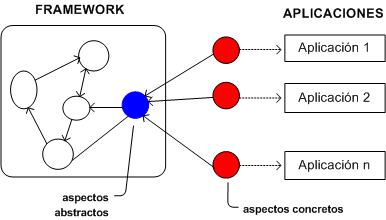
\includegraphics[scale=0.70]{figs/fig2.png}
	\caption{\label{fig:fig2} Esquema general del framework.}
\end{figure*}

\subsection{Requerimientos}
\label{subsec:requerimientos}
El framework ha sido construido desde cero aplicando un proceso iterativo de sucesivos refinamientos. Inicialmente se estableció el concepto y alcance de tarea. Definitivamente la tarea es un conjunto de acciones significativas para el evaluador que \colorbox{green}{ocurre-sucede} durante la ejecución de la aplicación. Sin embargo, este concepto no está representado como entidad del sistema, por ser un concepto subyacente y subjetivo. La tarea entonces debe ser representada en el framework, resultando esta abstracción de una relevancia central dado que todo el framework requiere mantener relaciones e interacciones que son dependientes de la misma. Desde esta visión una  tarea es una entidad subyacente a la aplicación que requiere encapsular un conjunto de estados y comportamiento interno,  puesto que realiza una o más operaciones y provee un comportamiento global para lograr el objetivo específico. Por lo cual, cualquier y toda tarea podrá ser relacionada con algún evento del sistema que establece su inicio y también con otro evento que indica su finalización. Una tarea podrá ser instanciada diversas veces en la misma o distintas ejecuciones de la aplicación (sesiones), cada instancia deberá ser identificable, ya que comporta diferentes valores para los estados descriptores. 

A partir del planteo de un escenario general y abstracto se ha procedido a identificar el conjunto de eventos que desencadenan las acciones que ejecutará y/o controlará el framework y el tipo de módulo (clase o aspecto) del framework que será responsable de ejecutar la función correspondiente (Tabla~\ref{tab:tab1}).  Los  eventos se clasifican en dos categorías según su origen. Los eventos de la aplicación (se ha producido un error mientras se ejecutaba la tarea) o los eventos pueden ser activados  por el mismo framework (se instancia una tarea). Asimismo un evento puede desencadenar una o más acciones, las cuales pueden ser llevadas a cabo por distintos módulos. 

%insert table1
% \usepackage{multirow}
\begin{table}[h]
\centering
\caption{Eventos-Acciones-Módulos}
\label{tab:tab1}
\begin{tabular}{|l|l|l|l|l|}
\hline
\multicolumn{2}{|c|}{Evento}                                                                                            & \multicolumn{2}{c|}{Acciones/Responsabilidad}                                              & \multicolumn{1}{c|}{Módulo} \\ \hline
\multirow{2}{*}{E1} & \multirow{2}{*}{\begin{tabular}[c]{@{}l@{}}Ejecución del \\ inicio de una tarea (D)\end{tabular}} & A1  & Interceptar inicio de una tarea                                                      & \multirow{2}{*}{Aspecto}    \\ \cline{3-4}
                    &                                                                                                   & A2  & Instanciar una tarea                                                                 &                             \\ \hline
\multirow{2}{*}{E2} & \multirow{2}{*}{Instanciar Tarea (F)}                                                             & A3  & Registrar inicio de la tarea                                                         & Clase                       \\ \cline{3-5} 
                    &                                                                                                   & A4  & Logging inicio de la tarea                                                           & Aspecto                     \\ \hline
\multirow{2}{*}{E3} & \multirow{2}{*}{\begin{tabular}[c]{@{}l@{}}Ejecución del \\ fin de una tarea (D)\end{tabular}}    & A5  & Interceptar el fin de una tarea                                                      & \multirow{2}{*}{Aspecto}    \\ \cline{3-4}
                    &                                                                                                   & A6  & Ordenar el fin de la tarea                                                           &                             \\ \hline
\multirow{3}{*}{E4} & \multirow{3}{*}{Se produce un error (D)}                                                          & A7 & Identificar el error                                                                  & \multirow{2}{*}{Aspecto}    \\ \cline{3-4} 
                    &                                                                                                   & A8 & Logging errores									     &  	   		   \\ \cline{3-5}
                    &                                                                                                   & A9 & Contabilizar error                                                                    & Clase                       \\ \hline
\multirow{3}{*}{E5} & \multirow{3}{*}{Finalizar la tarea (F)}                                                           & A10  & Registrar fin de la tarea                                                           & Clase    		   \\ \cline{3-5}
                    &                                                                                                   & A11  & \begin{tabular}[c]{@{}l@{}}Proporcionar el \\ Cuestionario Satisfacción\end{tabular}& \multirow{2}{*}{Aspecto}    \\ \cline{3-4}
                    &                                                                                                   & A12  & Logging Datos del fin de la tarea                                                   &     			   \\ \hline 
\end{tabular}
\end{table}

Los eventos E1 y E3, originados en el dominio (D), permiten identificar, delimitar y hacer el seguimiento de la tarea durante su tiempo de vida (ejecución), lo que implica que debidamente generarán las acciones de instanciación (A1-A2) y finalización(A5-A6), estas acciones serán llevadas a cabo por un aspecto. Al instanciar una tarea (E2) es necesario comenzar a registrar los datos (A3) que serán necesarios para el cálculo de métricas (duración) y accionar el log de la tarea (A4). En esta sucesión de eventos y acciones, el framework condiciona una cantidad de acciones a eventos internos que están supeditados a los cambios de la tarea. Esta premisa hace a los módulos del framework más independientes del dominio.

\subsection{Diseño e Implementación}
\label{subsec:disenio_e_implementacion}

En la Figura~\ref{fig:fig3} se presenta el diseño del framework, la implementación está desarrollada en Java y AspectJ. La clase Task constituye el núcleo del framework, dado que mantiene diversas relaciones con los restantes módulos. Los aspectos tienen un rol preponderante, ya que son necesarios para conectar la tarea con la aplicación y para comunicarla con otros servicios del framework (logging). El aspecto TaskConnect conecta a la tarea con los correspondientes eventos de inicio y finalización y realiza las acciones de crear la instancia de la Task y ordenar su finalización. El aspecto TaskError intercepta los errores que se producen en la ejecución de la tarea creada por TaskConnect y el aspecto TaskSatisfaction facilita un formulario que permite registrar la información subjetiva cuando la tarea ha sido finalizada. El aspecto TaskLog registra el logging de las tareas, cuando estas se crean, finalizan o generan otros eventos, de manera que es dependiente de la tarea y no de la aplicación. 
%insertar fig3
\begin{figure*}[ht!]
	\centering
	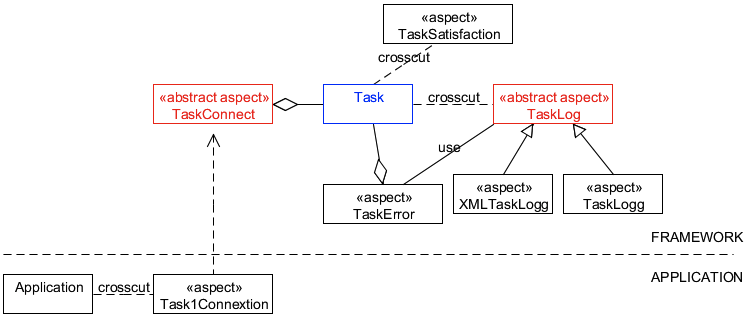
\includegraphics[scale=0.47]{figs/fig3.png}
	\caption{\label{fig:fig3}  Diseño del framework.}
\end{figure*}
A continuación se presenta los principales detalles del diseño interno e implementación de los módulos del framework. Cómo se mencionó la clase Task representa una tarea del usuario. Tiene diversos estados que permiten calcular posteriormente métricas o que van acumulando los valores de las mismas. Estos estados son inicializados en su instanciación. El atributo init se inicializa con la hora del sistema y el atributo complete con el valor falso. Estos dos atributos serán posteriormente actualizados por el método finalize (cuando la tarea finaliza) y usados para calcular el tiempo (eficiencia de la tarea) y si se ha completado (efectividad de la tarea). Para cada atributo que permite contabilizar errores como los atributos relacionados a la satisfacción existen métodos que permiten su correcta actualización. 

\begin{verbatim}
class Task  {
  private String id,
  private Time init, end;
  private boolean complete;
  private int #exception, sat1, sat2, sat3;
  Task(..){
     // inicialización de estados}
   …
  finalize()
    {// actualización de estados }
}
\end{verbatim}

El aspecto abstracto TaskConnect conecta la tarea con la aplicación. Dos pointcuts abstractos startTask y endTask son necesarios para definir los join-points (clase y método del dominio)  en los cuales comienza y finaliza cada tarea. Estos deberán ser definidos en un aspecto concreto por el desarrollador, que deberá crear un subaspecto por cada tarea de usuario distinta que pretenda evaluar. TaskConnect  tiene por atributo una tarea, (objeto  de tipo Task) que es instanciado por dicho aspecto cuando el pointcut startTask es activado y se ejecuta el aviso asociado, lo cual ocurre antes de que cada tarea inicie. De manera similar, este aspecto ordena la finalización de la tarea cuando luego que se activa el pointcut endTask, por medio del aviso asociado, se invoca al método.  

\begin{verbatim}
abstract aspect TaskConnect {
   private String idTask;
   private Task t;
   abstract pointcut starTask; 
   abstract pointcut endTask;
   before() : initTask();
   {  this.setTask();
      t = new Task(idTask);}
   after() : endTask()
   { t.finalize(); }
}
\end{verbatim}
El aspecto TaskError tiene por objeto interceptar los errores que se producen durante la ejecución de una tarea y ordenar la actualización de los acumuladores correspondientes de la tarea. El aspecto mantiene una referencia a la tarea instanciada, por medio del pointcut beginning y el atributo monitored\_task. Luego por cada tipo de error que se registra, se define un pointcut y advice. Tal es el caso del pointcut exception, cuyo objetivo es interceptar las excepciones que se producen mientras la tarea se ejecuta. Para ello es necesario especificar varias condiciones, que permiten delimitar al conjunto de excepciones que se producen. Estas restricciones debido a que también son necesarias para la intercepción de otros tipos errores se especifican en forma aislada e individual en los pointcuts condition\_1, condition\_2 y condition\_3. Luego en el pointcut exception se combinan con el descriptor de pointcut más específico, para este caso, handler. El advice asociado, primero actualiza el contador de excepciones de la tarea y luego ordena el log del error, operación que realiza el aspecto TaskLog. 
\begin{verbatim}
aspect TaskError {
  Task monitored_task=null;
  pointcut inicialization():    
               initialization(Task.new(String));
  pointcut beginning(Task t):inicialization()&&this(t);
  after(Task t): beginning(t)
    {monitored_task=t;} 
  pointcut condition_1():!cflow(adviceexecution)
  pointcut condition_2():!cflow(inicialization) 
  pointcut condition_3():if ((monitored_task!=null)&&
                            (!monitored_task.isComplete()))
  pointcut exception(Throwable e): 
                handler(Throwable+) && args(e)
                && condition_1() && condition_2()
                && condition_3()
  before(Throwable e): exception(e) {
     // actualizar monitored_task;
     TaskLog.aspectof().logException(e);
  }
}
\end{verbatim}
Cuando se produce la finalización de una tarea, (el método finalize de Task es invocado por el aspecto TaskConnect), el aspecto TaskSatisfaction proporciona un cuestionario que permite obtener información subjetiva del usuario relacionada a la dimensión satisfacción. Este formulario es muy simple, permite al usuario elegir un valor entre 1 y 5 para cada una de las 3 preguntas que se muestran en pantalla. 
\begin{verbatim}
aspect TaskSatisfaction {
   pointcut satisfaction(Task t):
        execution(void Task.finalize(..))&&this(t);	
   before(Task t): satisfaction (t) {
	// desplegar cuestionario 
       // obtener datos ingresados por el usuario.
	// actualizar atrubutos sat1..de t
   return;}
}
\end{verbatim}
Finalmente el aspecto TaskLog  realiza el logging de la tarea en diversos momentos. Es una aspecto abstracto debido a que el log puede realizarse en diversos formatos (texto / xml / base de datos / consola). Los pointcut están definidos de manera concreta, ya que este aspecto está supeditado por completo a los cambios en la tarea.  
\begin{verbatim}
abstract aspect TaskLog {
   abstract void logException() // log de excepciones
   abstract void logTask() 
   pointcut logSart(Task): call Task.new(..) && target(t);
   pointcut logEnd(Task): call Task.finalize(..) && target(t);
   after() : logStart()
   { logTask(t);}
   after() : logEnd()
   { logTask(t);}
}
\end{verbatim}
El diseño e implementación de los módulos del framework se ha apoyado en distintos patrones de diseño aspectuales~\cite{HS2003}. Por ejemplo, en el caso de TaskConnect se aplicaron los patrones Abstract Pointcut y Template Advice, en TaskError se aplicó el patrón Composite Pointcut y en TaskLog se aplicó el patrón Template Advice.

\section{Casos de Estudio}
\label{sec:casos_de_estudio}
 
 El desarrollo iterativo del framework implicó la ejecución de pruebas con cada versión del framework obtenida. El mismo ha sido probado y validado empleando dos aplicaciones de escritorio JMoney (http://jmoney.sourceforge.net/) y Freemind (http://freemind.sourceforge.net/). 
 
%\begin{description}
%
%\item[JMoney]
%
%%Es un gestor de finanzas de uso personal. Tiene ??? paquetes, 83 clases, 594 métodos y 436 atributos. Se compone de 5780 líneas de código. 
%
%\item[Freemind]
%
%%Es una herramienta para la creación de mapas mentales. Tiene 50 paquetes, 820 clases, 6974 métodos, 2816 atributos. Se compone de 108.378 líneas de código. 
%\end{description}

Para cada una se crearon diversas tareas y en cada iteración se configuró el framework. Los principales objetivos de las pruebas fueron constatar que el registro de los datos y cálculo de las métricas funcionaba correctamente; y comprobar el nivel de reúso, configuración y especialización. A continuación se presenta una tarea para cada caso de estudio, el aspecto que fue adaptado  y el resultado de las pruebas.


\begin{description}

\item[Freemind]
Tarea: Crear Mapa Mental Básico.

	\begin{enumerate}
		\item Crear un nuevo mapa, haciendo clic en el botón "Nuevo" desde la barra de herramientas, o desde el menú Archivo. 
		\item Completar el texto del nodo raíz del mapa creado.
		\item Construir una jerarquía de tres niveles con nodos hijos y hermanos (al menos 11).Para ello se deberá posicionar en el nodo sobre el cual quiere crear un nodo hijo o hermano y luego insertar el nodo desde las opciones del menú contextual, o desde el menú Insertar.
		\item Ir al menú herramientas y ordenar los nodos por nombre.
		\item Guardar el mapa mental en el escritorio con un nombre significativo.
	\end{enumerate}
	
%	\begin{itemize}
%		\item Inicio de la tarea: La tarea se considerará iniciada luego que el usuario haya seleccionado la opción "Nuevo Mapa" del menú principal o desde la barra de herramientas.
%		\item Fin de la tarea: La tarea se considerará finalizada luego que el usuario guarda, por primera vez, el mapa en un archivo con el nombre solicitado. 
%	\end{itemize}
	
	\begin{verbatim}
	public aspect FreemindTask1extends TaskConnect{
	 private String idTask="Crear Mapa Conceptual Básico”;
	 pointcut startTask():execution(void  
	 freemind.modes.common.actions.NewMapAction.	\\
	 actionPerformed(ActionEvent));
	 pointcut endTask():execution( 	 
	  *freemind.modes.ControllerAdapter.SaveAsAction.*(..)) ||
	    execution(* freemind.modes.ControllerAdapter.\\
	    SaveAction.*(..));
	}
	\end{verbatim}

	%insertar fig4.png
	\begin{figure*}[ht!]
		\centering
		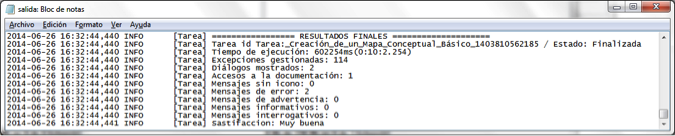
\includegraphics[scale=1]{figs/fig4.png}
		\caption{\label{fig:fig4} Log de Tarea: Crear Mapa Conceptual Básico.}
	\end{figure*}

\item[JMoney]
Tarea: Crear una nueva cuenta

	\begin{enumerate}
		\item Hacer click en el botón derecho del panel lateral y seleccionar la opción "new account".
		\item Ingresar las propiedades de la cuenta desde el panel properties de la cuenta
		\item Ingresar entradas en la cuenta desde el panel entries  
		\item Salvar desde el botón "save" en la barra de herramientas o desde menú "file/save", usando combinación de teclas "ctrl+s" o respondiendo afirmativamente al mensaje de grabar los cambios antes de cerrar la aplicación.
	\end{enumerate}

	\begin{verbatim}
		public aspect Tarea1JMoneyConnect extends TareaConnect{		
		     private String idTask=”Crear Nueva Nuenta”;
		     pointcut starTask():execution(void   
		                  net.sf.jmoney.gui.MainFrame.newAccount());
		     pointcut endTask():execution(void                  
		               net.sf.jmoney.gui.MainFrame.saveSession()) || 
		       execution(void net.sf.jmoney.gui.MainFrame.saveSessionAs());
	}
	\end{verbatim}

	%insertar fig5.png
	\begin{figure*}[ht!]
		\centering
		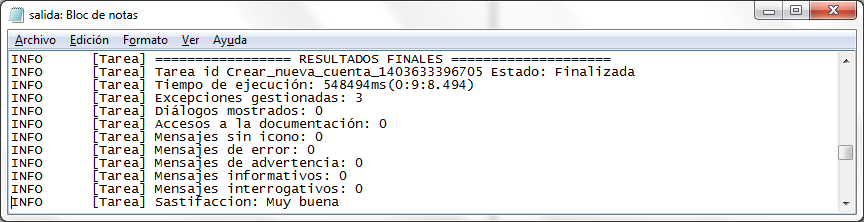
\includegraphics[scale=1]{figs/fig5.png}
		\caption{\label{fig:fig5} Log de Tarea: Crear Nueva Cuenta.}
	\end{figure*}
	
\end{description}

\section{Trabajos Relacionados}
\label{sec:trabajos_relacionados}
Como se mencionó anteriormente, existen contribuciones que aplican AOP para la evaluación de la usabilidad de aplicaciones de escritorio~\cite{TM2006,ST2010,HBS2011,TAO2008,TAO2012,BGO+2009,HDC2009}. La principal diferencia con estos trabajos es que no distinguen a la Tarea entre los aspectos. Los aspectos hacen el seguimiento de eventos y registran datos simplemente. Se requiere mayor intervención del desarrollador, es decir, son esquemas menos reusables y flexibles.

%Tarta y Moldovan~\cite{TM2006} proponen un diseño de aspectos que soporta la evaluación automática de la usabilidad en aplicaciones de escritorio. Se plantea que mediante una jerarquía de aspectos se pueden reusar pointcuts que compartan los mismos puntos de entrada y salida (join-points). Los aspectos derivados definen nuevos pointcuts para la intercepción de errores, completitud de tareas, captura de pantallas y adquisición de datos por medio de cuestionarios. Los aspectos concretos por medio de los advices realizan el log de los datos. Aquí los aspectos hacen el seguimiento y el logging en el mismo aspecto pero en reiteradas veces dado que existen aspectos para los errores, el cálculo del tiempo, etc. y por ende el desarrollador debe configurar más aspectos, pero se pierde la noción de la tarea, por lo que toda la estructura es específica de cada aplicación en la que se use. Se presentan simples diagramas y código de ejemplo en AspectJ.

%Shekh y Tyerman~\cite{ST2010} presentan el desarrollo de un framework AOP para la evaluación de la usabilidad con AOP. Las autoras registran los eventos de UI, por ejemplo los eventos del mouse. Respecto de las características del framework y diseño de aspectos no se brindan detalles, pero se indica que han seguido las recomendaciones de~\cite{TM2006}. El framework está desarrollado en AspectJ. Se presentan resultados de experimentos controlados y pautados en un laboratorio.

%Holzinger y otros~\cite{HBS2011} proponen la implementación de aspectos para seguir la trayectoria de algunos eventos de interface (entrada del teclado, menúes y acciones arrastrar y soltar). Se plantea usar Objective-C, agregando los aspectos a la jerarquía de objetos usando la tecnología “método swizzling”, y extendiendo de clases. El diseño se centra en un aspecto que realiza el logging de manera centralizada y tres aspectos son necesarios para identificar los eventos de interface mencionados. 

%Tao~\cite{TAO2008} propone AOP para capturar automáticamente eventos de la interfaz de usuario en aplicaciones con arquitectura MVC (modelo-vista-controlador). Se propone una jerarquía de aspectos, en la cual se logra reusar solo el método que realiza el reporte (hora-fecha y evento ocurrido), los pointcuts y advices deben ser redefinidos en cada caso y aplicación, por ejemplo actualización de observador, manejadores y notificadores de eventos, cuadros de diálogo. Se presentan códigos de ejemplo en AspectJ y un caso de estudio simple.
  
%Un esquema muy similar al anterior, es el que presenta Tao~\cite{TAO2012}, ya que este enfoque se basa en técnicas AO para ejecutar las trazas de los eventos de interfaz de usuario y recolectar información contextual, en aplicaciones de escritorio (WIMP). Propone una jerarquía de aspectos, la cual consiste básicamente en un método  que contiene la lógica que permite hacer el reporte, los sub-aspectos definen los eventos a interceptar en los pointcuts y los advice que invocan al método que ejecuta el reporte. Se presentan simples códigos de ejemplo en AspectJ.

%Bateman y otros~\cite{BGO+2009}presentan el enfoque “Instrumentación Interactiva de Usabilidad” (IIU). Los evaluadores de usabilidad especifican qué acciones serán registradas (log) interactuando con los elementos de la interfaz de la aplicación objeto de la evaluación, eliminando la necesidad de apoyo adicional de programación. Esta primera actividad se apoya en AOP, y permite la instrumentación a través de la interacción directa con la aplicación a ser instrumentada; se decide qué elementos (interfaz) de un sistema están relacionados con tareas particulares y problemas de usabilidad. 

%Humayoun y otros~\cite{HDC2009} presentan la herramienta UEMan que permite gestionar y automatizar actividades de la evaluación de la usabilidad desde un enfoque UCD (diseño centrado en el usuario) durante el proceso de desarrollo de software. El modelo y la herramienta incorporan el concepto de tarea de usuario y facilita la ejecución de diversos tipos de experimentos: de evaluación heurística, de tipo tarea, basados en cuestionarios y experimentos dinámicos que emplean logging implementado con aspectos. La herramienta usa aspectos para operaciones muy básicas como, hacer el Timer (duración) de una actividad (desde un punto de entrada hasta un punto de salida, definido mediante dos pointcuts) y contar la cantidad de clicks del mouse y teclas presionadas en dicho intervalo.


\section{Conclusiones}
\label{sec:conclusiones}
En este trabajo se ha presentado un framework que permite la evaluación de la usabilidad de aplicaciones de escritos de alto nivel, dado que permite obtener información y calcular métricas a nivel de tareas de usuario, en las dimensiones de eficiencia, efectividad y satisfacción. El framework automatiza la recolección de datos y algunas funciones de análisis. Aunque el framework se compone de varios módulos, el desarrollador sólo debe configurar dos pointcut de un solo aspecto (TaskConnect), para que toda la evaluación de usabilidad de una determinada tarea sea efectuada. Lo cual implica un alto nivel de reúso, del diseño y la implementación, ya que se ha logrado reducir al mínimo las condiciones de variación del problema y requerimientos de configuración. 
Los trabajos futuros refieren a incorporar más funcionalidad para la registración de otros datos relacionados a la tarea con el objeto de calcular nuevas métricas. También resulta de utilidad incorporar un visor que facilite la tarea de análisis y crítica posterior al evaluador de usabilidad. Completadas estas mejoras, el paso siguiente es desarrollar y evaluar un framework para aplicaciones web.


%-------------------------------------------------------------------------------
\bibliographystyle{splncs03}
\bibliography{bib}

\end{document}
